\section{GMI SRF Data Plots}
%===========================
\label{app.srf_data_plots}
\newpage

\addcontentsline{toc}{subsection}{Channel 1}
\begin{figure}[htp]
  \centering
  \begin{tabular}{c c}
    \includegraphics[scale=0.3]{graphics/lin/gmi_gpm-1.eps} &
    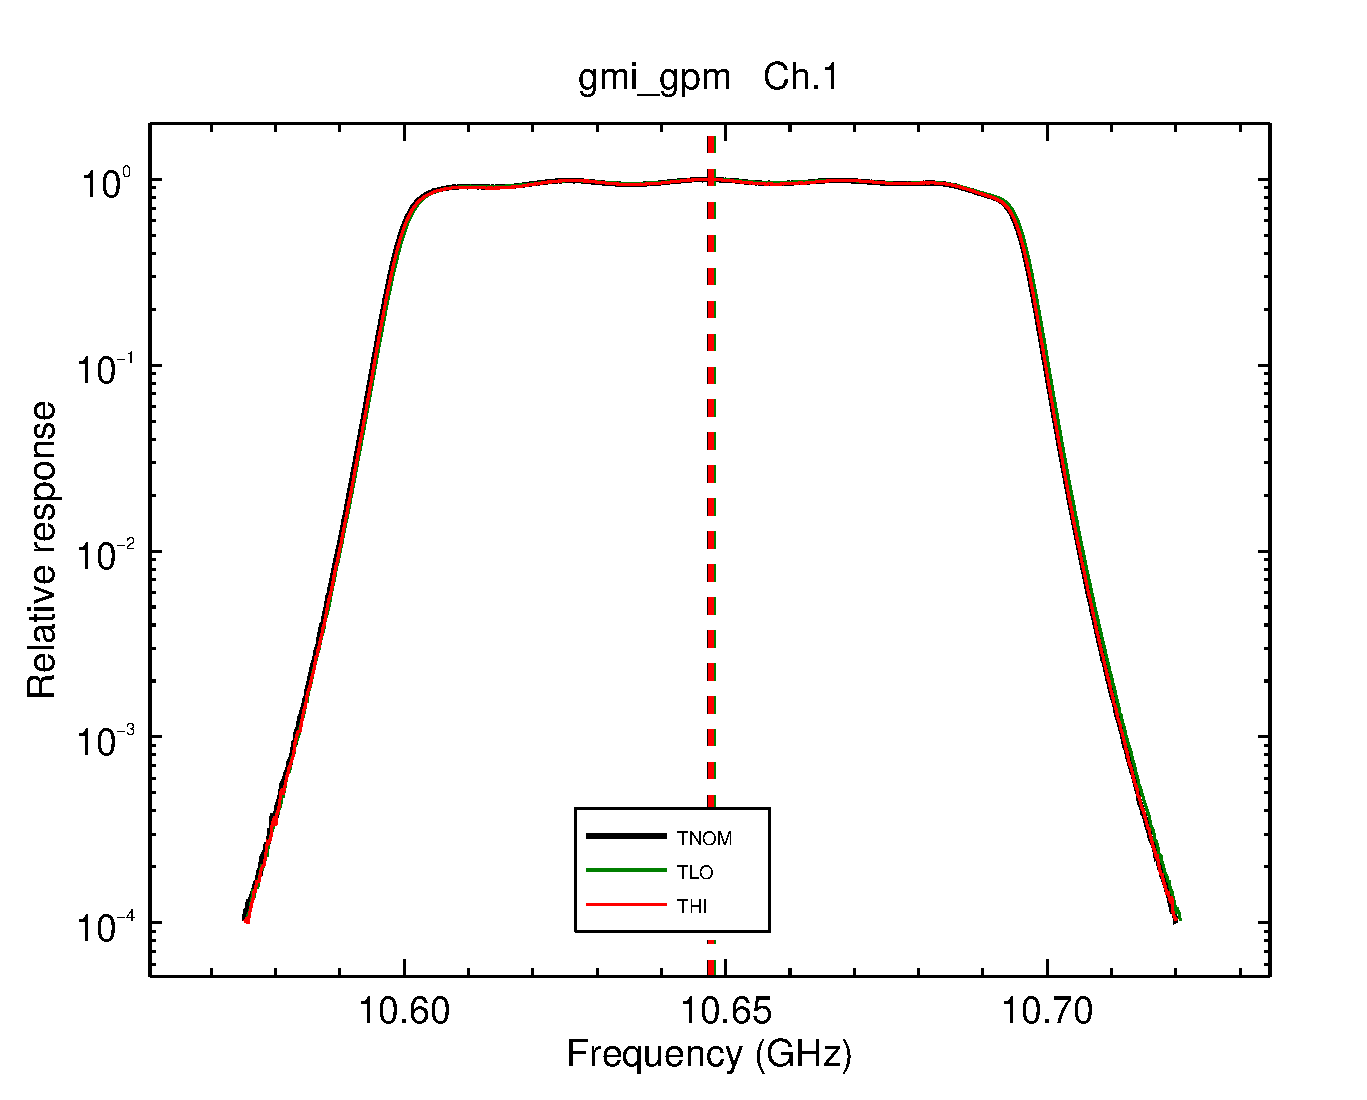
\includegraphics[scale=0.3]{graphics/log/gmi_gpm-1.eps}
  \end{tabular}
  \caption{GMI channel 1 responses for the three test temperatures: $T_{NOM}$ (25\textdegree{}C), $T_{LO}$ (-10\textdegree{}C), and $T_{HI}$ (45\textdegree{}C). Vertical dashed lines are the locations of the computed central frequencies. \textbf{(Left)} Linear y-axis. \textbf{(Right)} Base-10 logarithmic y-axis.}
  \label{fig:ch1_response}
\end{figure}

\addcontentsline{toc}{subsection}{Channel 2}
\begin{figure}[htp]
  \centering
  \begin{tabular}{c c}
    \includegraphics[scale=0.3]{graphics/lin/gmi_gpm-2.eps} &
    \includegraphics[scale=0.3]{graphics/log/gmi_gpm-2.eps}
  \end{tabular}
  \caption{GMI channel 2 responses for the three test temperatures: $T_{NOM}$ (25\textdegree{}C), $T_{LO}$ (-10\textdegree{}C), and $T_{HI}$ (45\textdegree{}C). Vertical dashed lines are the locations of the computed central frequencies. \textbf{(Left)} Linear y-axis. \textbf{(Right)} Base-10 logarithmic y-axis.}
  \label{fig:ch2_response}
\end{figure}

\addcontentsline{toc}{subsection}{Channel 3}
\begin{figure}[htp]
  \centering
  \begin{tabular}{c c}
    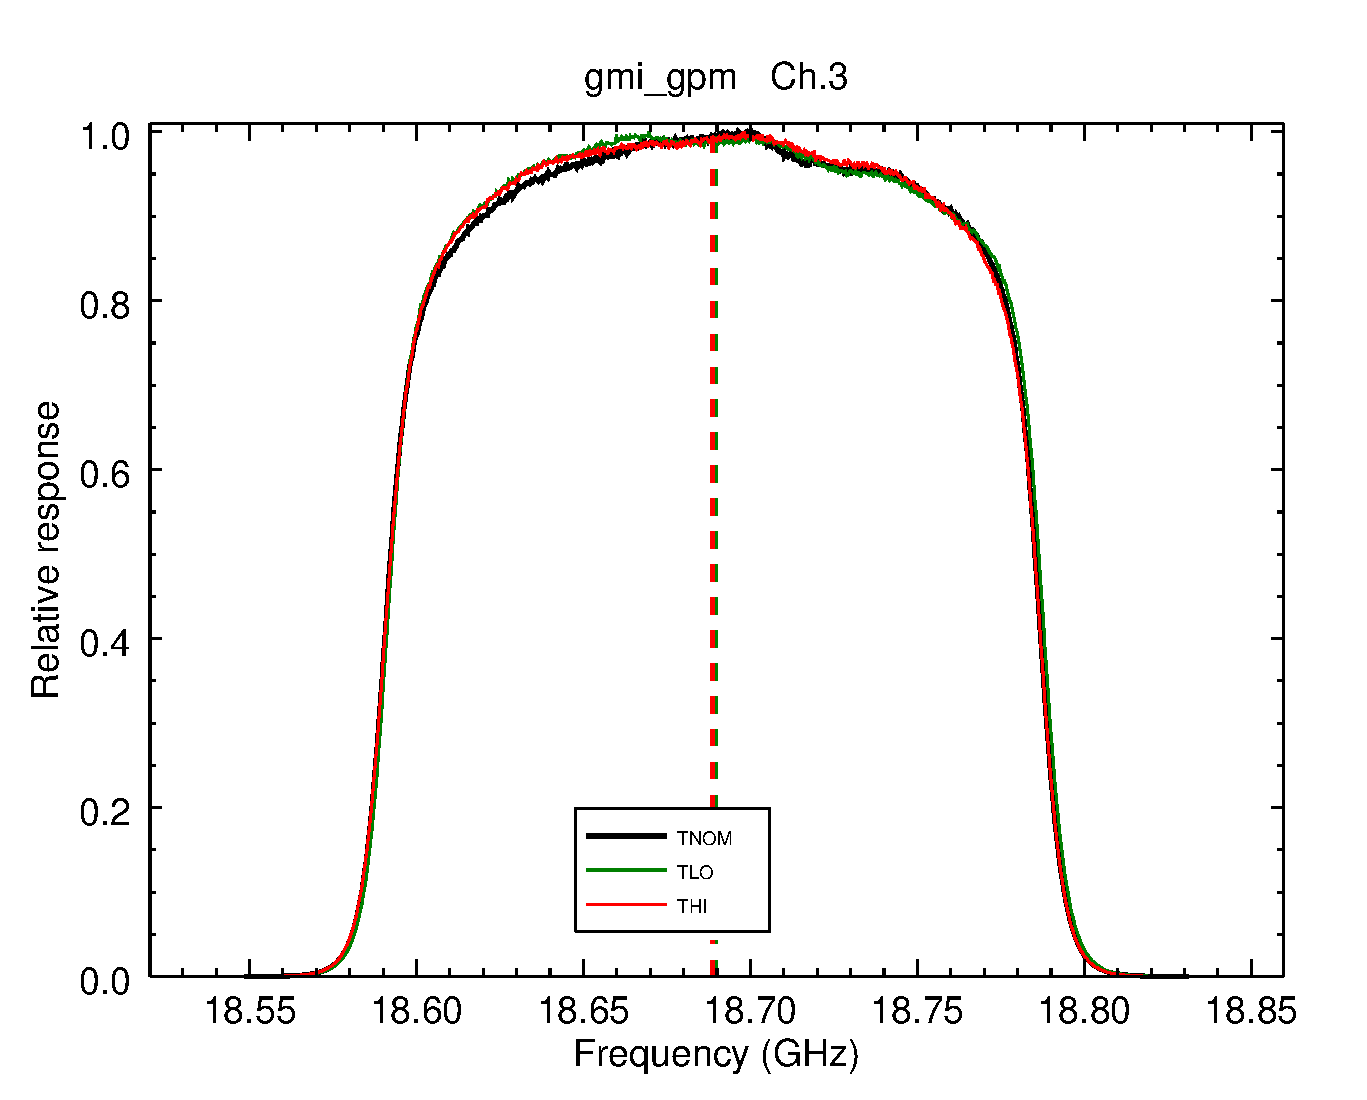
\includegraphics[scale=0.3]{graphics/lin/gmi_gpm-3.eps} &
    \includegraphics[scale=0.3]{graphics/log/gmi_gpm-3.eps}
  \end{tabular}
  \caption{GMI channel 3 responses for the three test temperatures: $T_{NOM}$ (25\textdegree{}C), $T_{LO}$ (-10\textdegree{}C), and $T_{HI}$ (45\textdegree{}C). Vertical dashed lines are the locations of the computed central frequencies. \textbf{(Left)} Linear y-axis. \textbf{(Right)} Base-10 logarithmic y-axis.}
  \label{fig:ch3_response}
\end{figure}

\addcontentsline{toc}{subsection}{Channel 4}
\begin{figure}[htp]
  \centering
  \begin{tabular}{c c}
    \includegraphics[scale=0.3]{graphics/lin/gmi_gpm-4.eps} &
    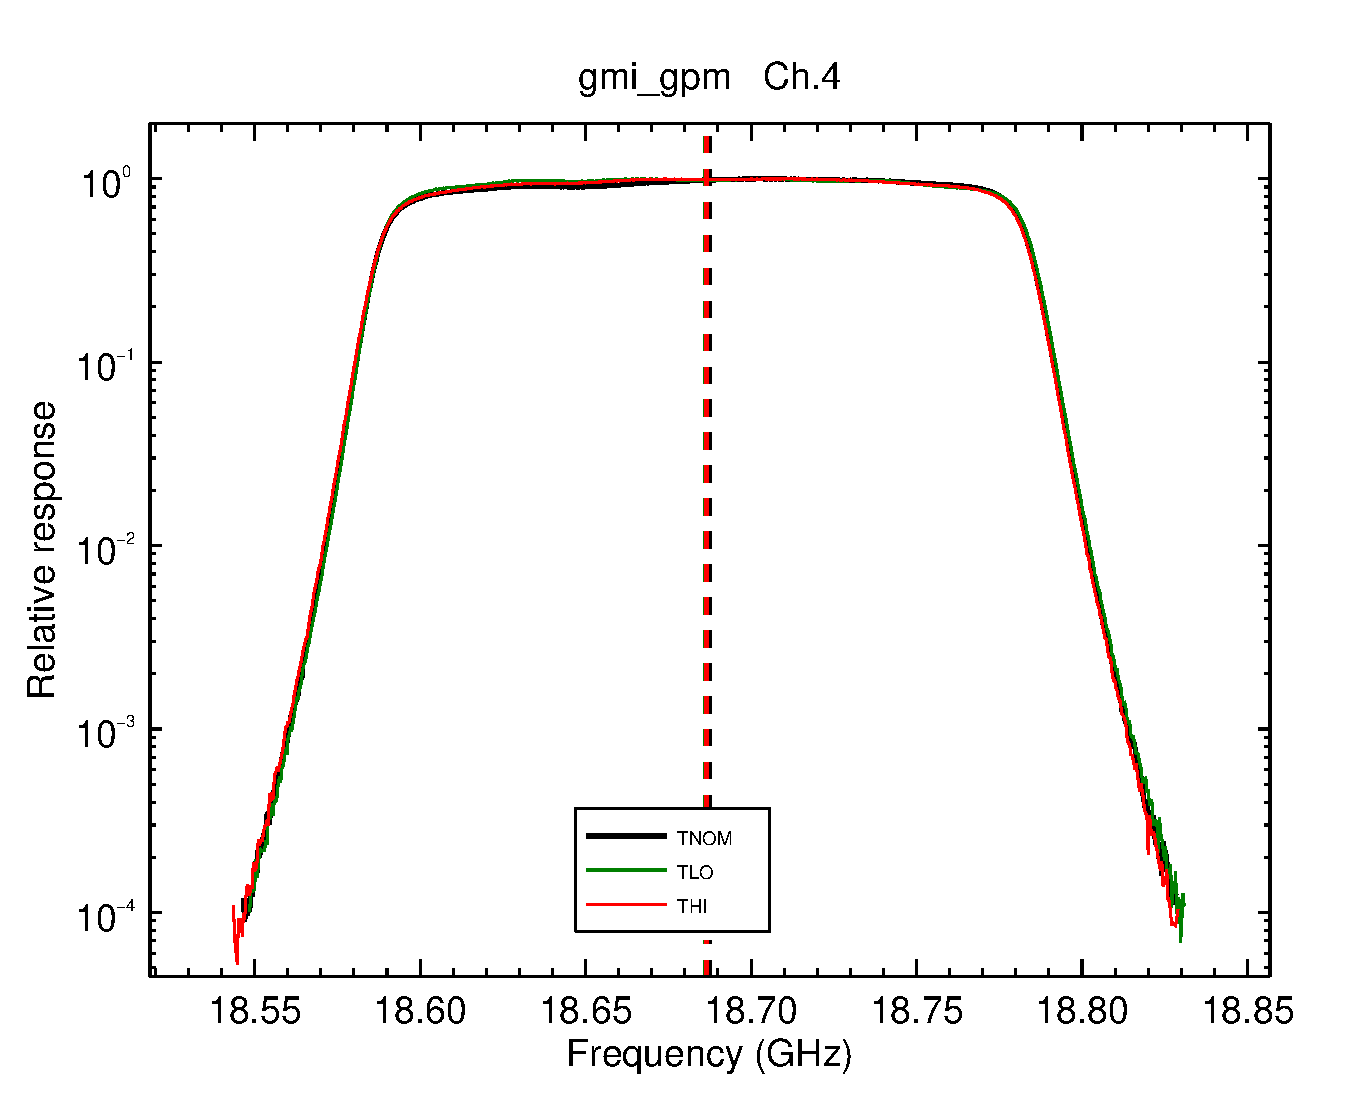
\includegraphics[scale=0.3]{graphics/log/gmi_gpm-4.eps}
  \end{tabular}
  \caption{GMI channel 4 responses for the three test temperatures: $T_{NOM}$ (25\textdegree{}C), $T_{LO}$ (-10\textdegree{}C), and $T_{HI}$ (45\textdegree{}C). Vertical dashed lines are the locations of the computed central frequencies. \textbf{(Left)} Linear y-axis. \textbf{(Right)} Base-10 logarithmic y-axis.}
  \label{fig:ch4_response}
\end{figure}

\addcontentsline{toc}{subsection}{Channel 5}
\begin{figure}[htp]
  \centering
  \begin{tabular}{c c}
    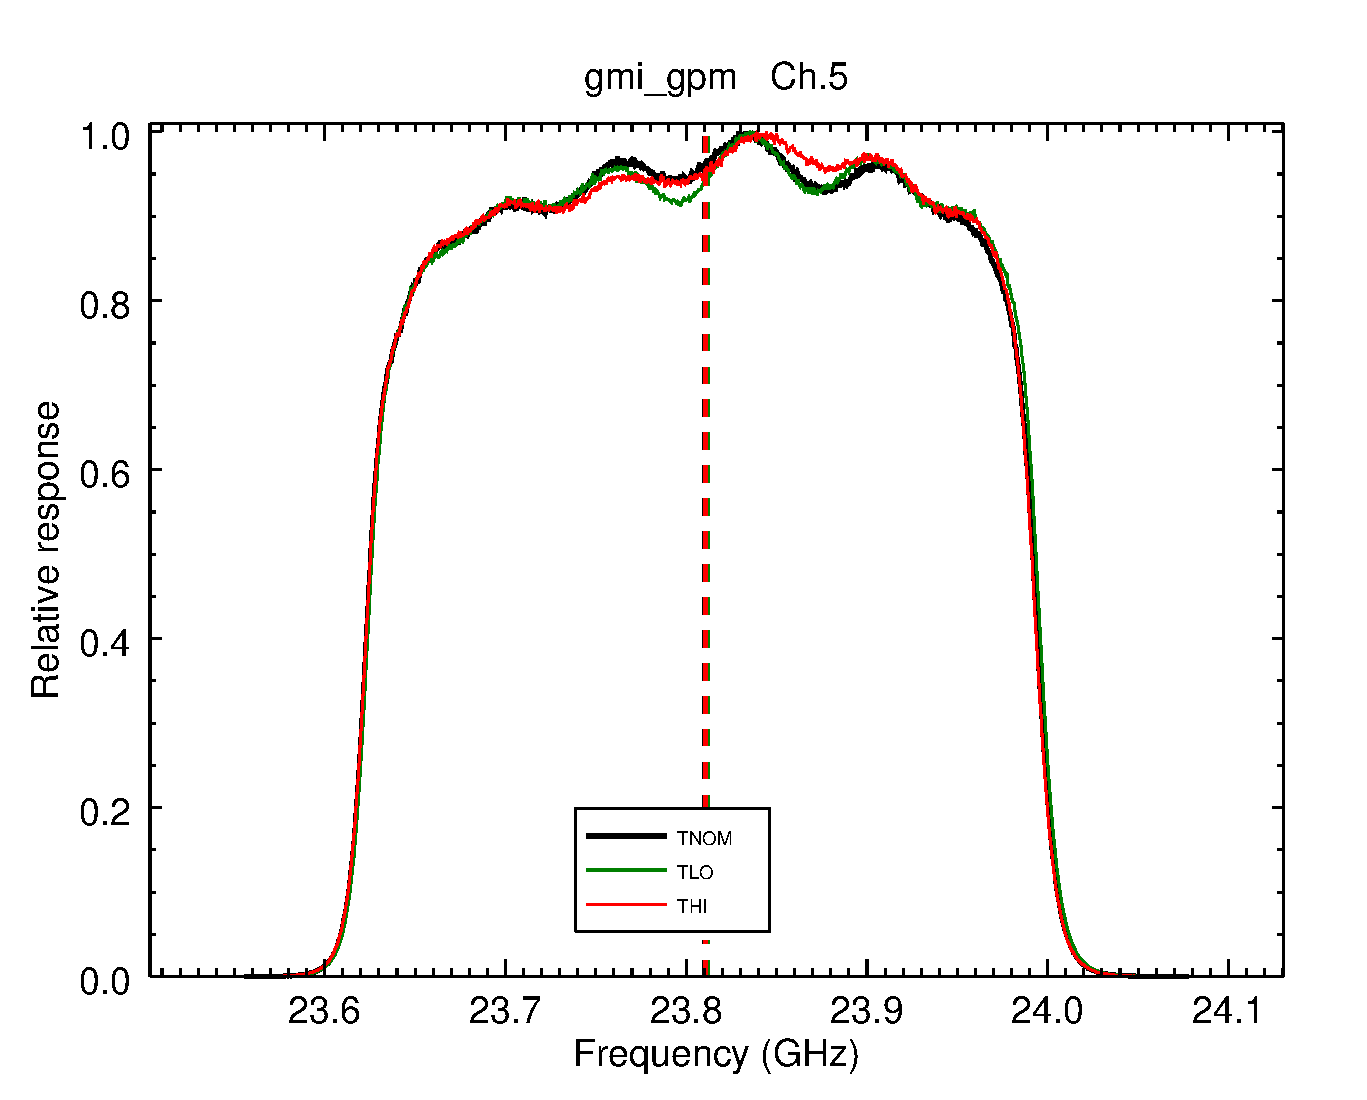
\includegraphics[scale=0.3]{graphics/lin/gmi_gpm-5.eps} &
    \includegraphics[scale=0.3]{graphics/log/gmi_gpm-5.eps}
  \end{tabular}
  \caption{GMI channel 5 responses for the three test temperatures: $T_{NOM}$ (25\textdegree{}C), $T_{LO}$ (-10\textdegree{}C), and $T_{HI}$ (45\textdegree{}C). Vertical dashed lines are the locations of the computed central frequencies. \textbf{(Left)} Linear y-axis. \textbf{(Right)} Base-10 logarithmic y-axis.}
  \label{fig:ch5_response}
\end{figure}

\addcontentsline{toc}{subsection}{Channel 6}
\begin{figure}[htp]
  \centering
  \begin{tabular}{c c}
    \includegraphics[scale=0.3]{graphics/lin/gmi_gpm-6.eps} &
    \includegraphics[scale=0.3]{graphics/log/gmi_gpm-6.eps}
  \end{tabular}
  \caption{GMI channel 6 responses for the three test temperatures: $T_{NOM}$ (25\textdegree{}C), $T_{LO}$ (-10\textdegree{}C), and $T_{HI}$ (45\textdegree{}C). Vertical dashed lines are the locations of the computed central frequencies. \textbf{(Left)} Linear y-axis. \textbf{(Right)} Base-10 logarithmic y-axis.}
  \label{fig:ch6_response}
\end{figure}

\addcontentsline{toc}{subsection}{Channel 7}
\begin{figure}[htp]
  \centering
  \begin{tabular}{c c}
    \includegraphics[scale=0.3]{graphics/lin/gmi_gpm-7.eps} &
    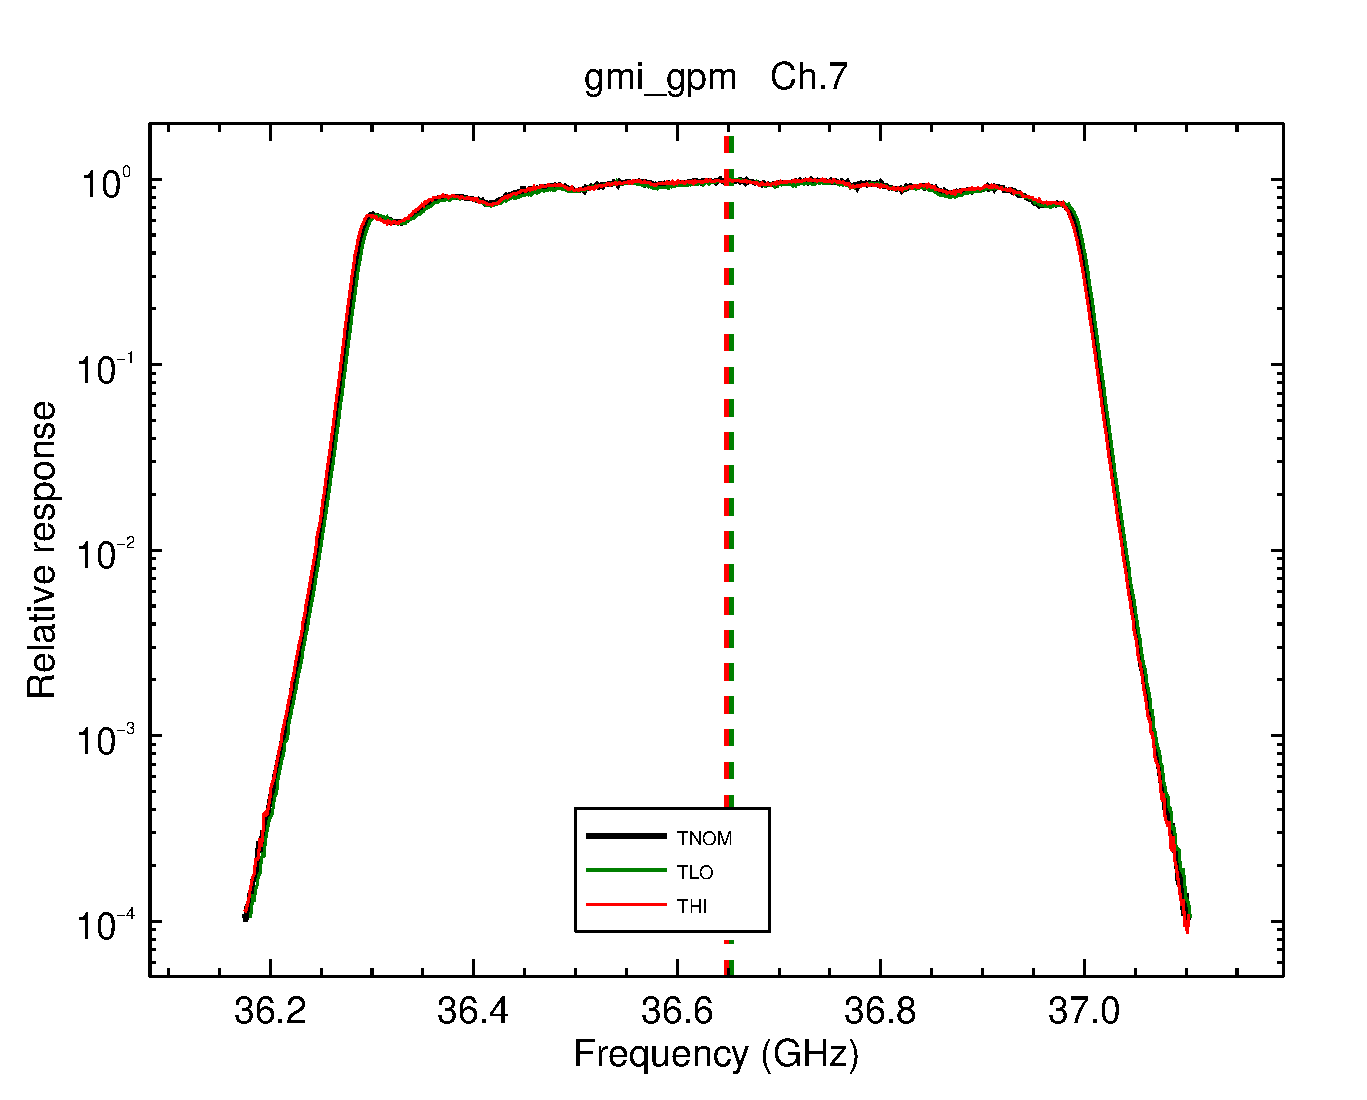
\includegraphics[scale=0.3]{graphics/log/gmi_gpm-7.eps}
  \end{tabular}
  \caption{GMI channel 7 responses for the three test temperatures: $T_{NOM}$ (25\textdegree{}C), $T_{LO}$ (-10\textdegree{}C), and $T_{HI}$ (45\textdegree{}C). Vertical dashed lines are the locations of the computed central frequencies. \textbf{(Left)} Linear y-axis. \textbf{(Right)} Base-10 logarithmic y-axis.}
  \label{fig:ch7_response}
\end{figure}

\addcontentsline{toc}{subsection}{Channel 8}
\begin{figure}[htp]
  \centering
  \begin{tabular}{c c}
    \includegraphics[scale=0.3]{graphics/lin/gmi_gpm-8.eps} &
    \includegraphics[scale=0.3]{graphics/log/gmi_gpm-8.eps}
  \end{tabular}
  \caption{GMI channel 8 responses for the three test temperatures: $T_{NOM}$ (25\textdegree{}C), $T_{LO}$ (-10\textdegree{}C), and $T_{HI}$ (45\textdegree{}C). \textbf{(Left)} Linear y-axis. \textbf{(Right)} Base-10 logarithmic y-axis.}
  \label{fig:ch8_response}
\end{figure}

\addcontentsline{toc}{subsection}{Channel 9}
\begin{figure}[htp]
  \centering
  \begin{tabular}{c c}
    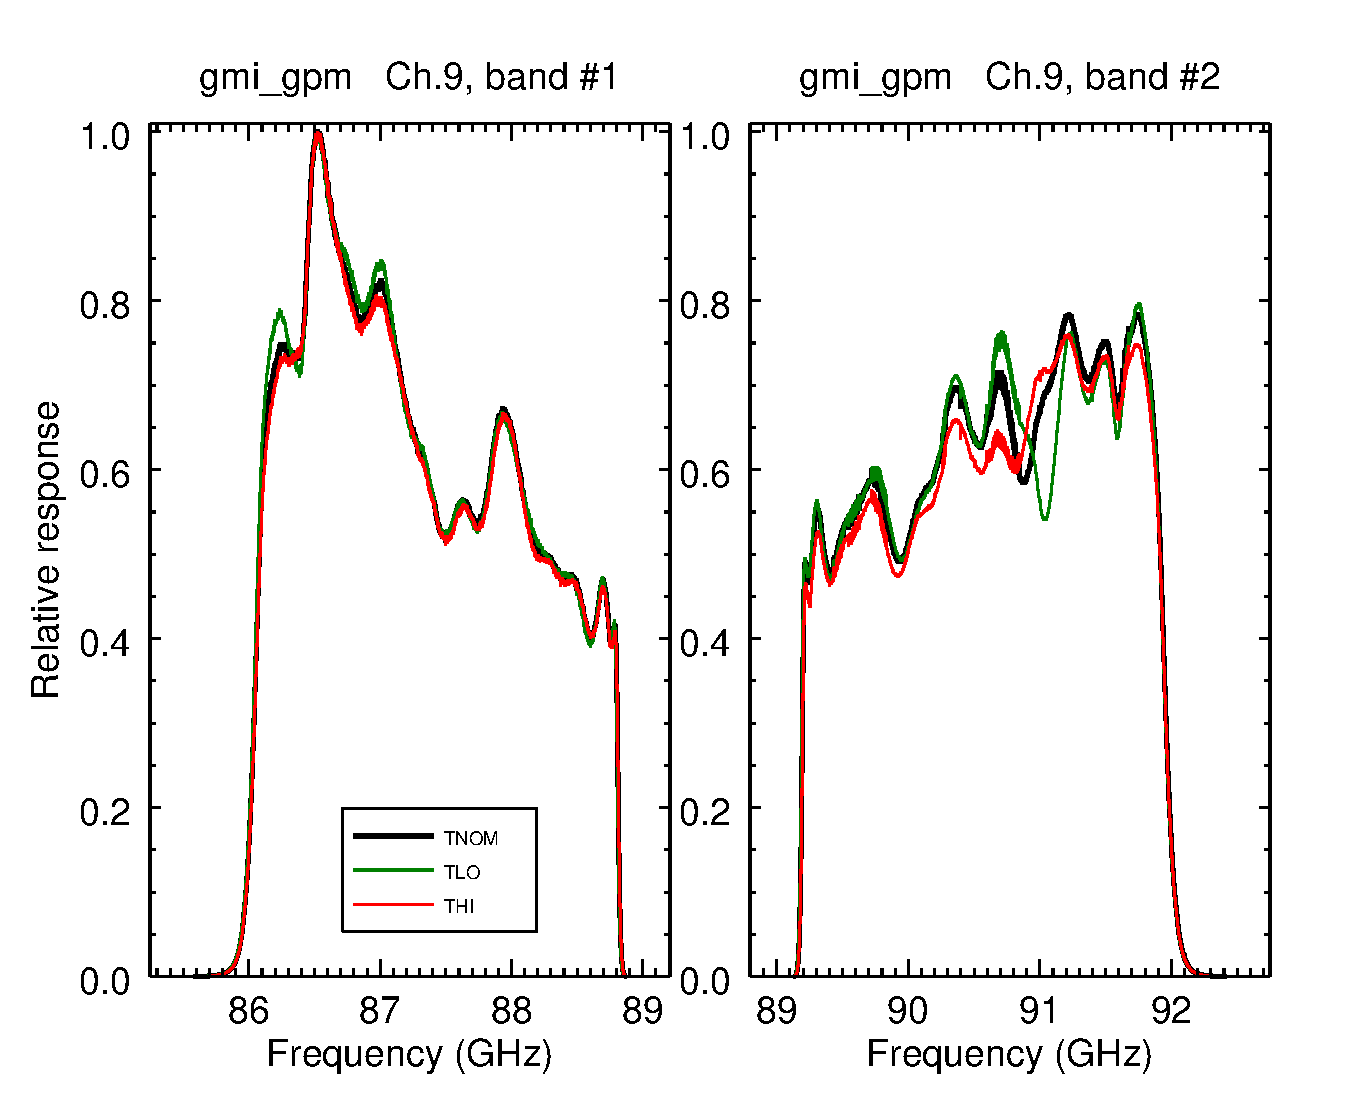
\includegraphics[scale=0.3]{graphics/lin/gmi_gpm-9.eps} &
    \includegraphics[scale=0.3]{graphics/log/gmi_gpm-9.eps}
  \end{tabular}
  \caption{GMI channel 9 responses for the three test temperatures: $T_{NOM}$ (25\textdegree{}C), $T_{LO}$ (-10\textdegree{}C), and $T_{HI}$ (45\textdegree{}C). \textbf{(Left)} Linear y-axis. \textbf{(Right)} Base-10 logarithmic y-axis.}
  \label{fig:ch9_response}
\end{figure}

\addcontentsline{toc}{subsection}{Channel 10}
\begin{figure}[htp]
  \centering
  \begin{tabular}{c c}
    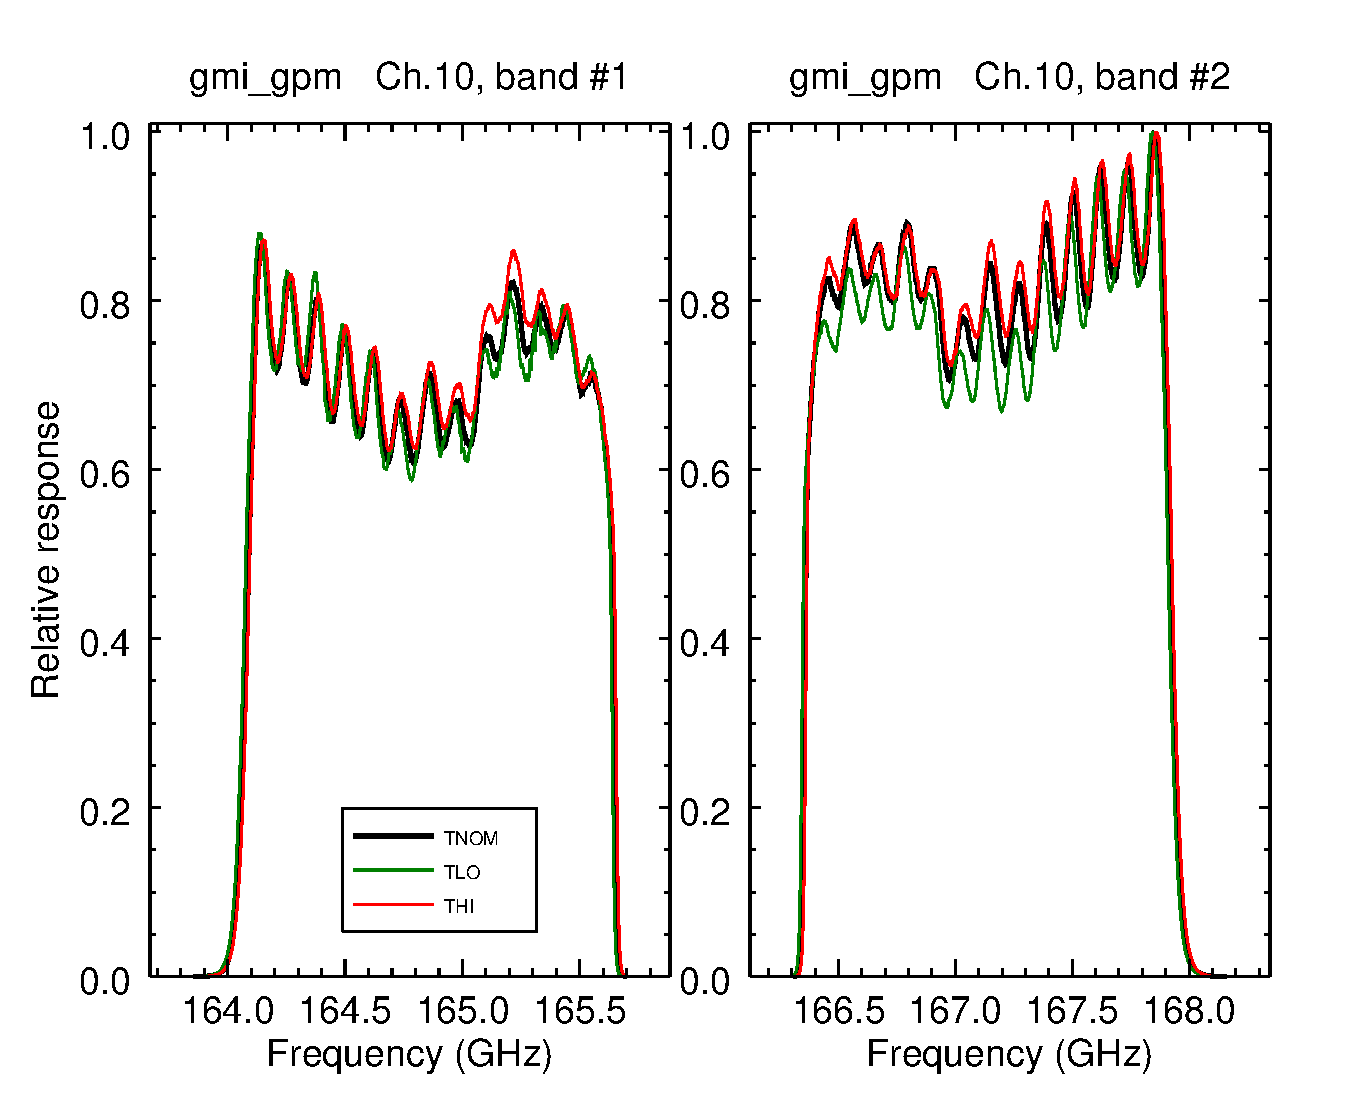
\includegraphics[scale=0.3]{graphics/lin/gmi_gpm-10.eps} &
    \includegraphics[scale=0.3]{graphics/log/gmi_gpm-10.eps}
  \end{tabular}
  \caption{GMI channel 10 responses for the three test temperatures: $T_{NOM}$ (25\textdegree{}C), $T_{LO}$ (-10\textdegree{}C), and $T_{HI}$ (45\textdegree{}C). \textbf{(Left)} Linear y-axis. \textbf{(Right)} Base-10 logarithmic y-axis.}
  \label{fig:ch10_response}
\end{figure}

\addcontentsline{toc}{subsection}{Channel 11}
\begin{figure}[htp]
  \centering
  \begin{tabular}{c c}
    \includegraphics[scale=0.3]{graphics/lin/gmi_gpm-11.eps} &
    \includegraphics[scale=0.3]{graphics/log/gmi_gpm-11.eps}
  \end{tabular}
  \caption{GMI channel 11 responses for the three test temperatures: $T_{NOM}$ (25\textdegree{}C), $T_{LO}$ (-10\textdegree{}C), and $T_{HI}$ (45\textdegree{}C). \textbf{(Left)} Linear y-axis. \textbf{(Right)} Base-10 logarithmic y-axis.}
  \label{fig:ch11_response}
\end{figure}

\addcontentsline{toc}{subsection}{Channel 12}
\begin{figure}[htp]
  \centering
  \begin{tabular}{c c}
    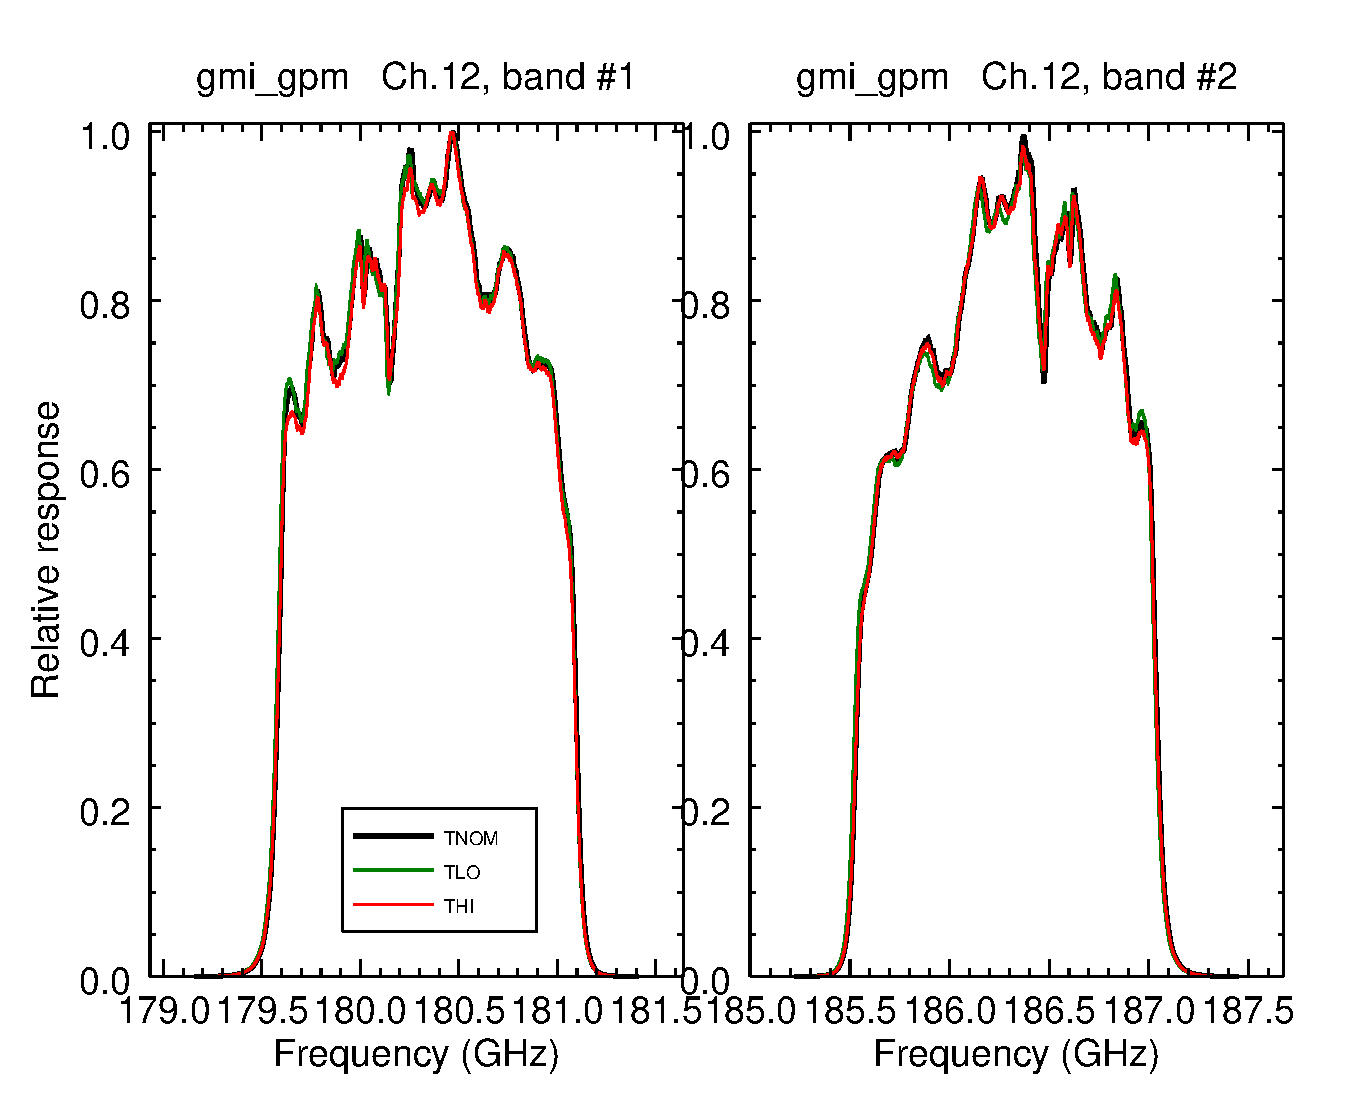
\includegraphics[scale=0.3]{graphics/lin/gmi_gpm-12.eps} &
    \includegraphics[scale=0.3]{graphics/log/gmi_gpm-12.eps}
  \end{tabular}
  \caption{GMI channel 12 responses for the three test temperatures: $T_{NOM}$ (25\textdegree{}C), $T_{LO}$ (-10\textdegree{}C), and $T_{HI}$ (45\textdegree{}C). \textbf{(Left)} Linear y-axis. \textbf{(Right)} Base-10 logarithmic y-axis.}
  \label{fig:ch12_response}
\end{figure}

\addcontentsline{toc}{subsection}{Channel 13}
\begin{figure}[htp]
  \centering
  \begin{tabular}{c c}
    \includegraphics[scale=0.3]{graphics/lin/gmi_gpm-13.eps} &
    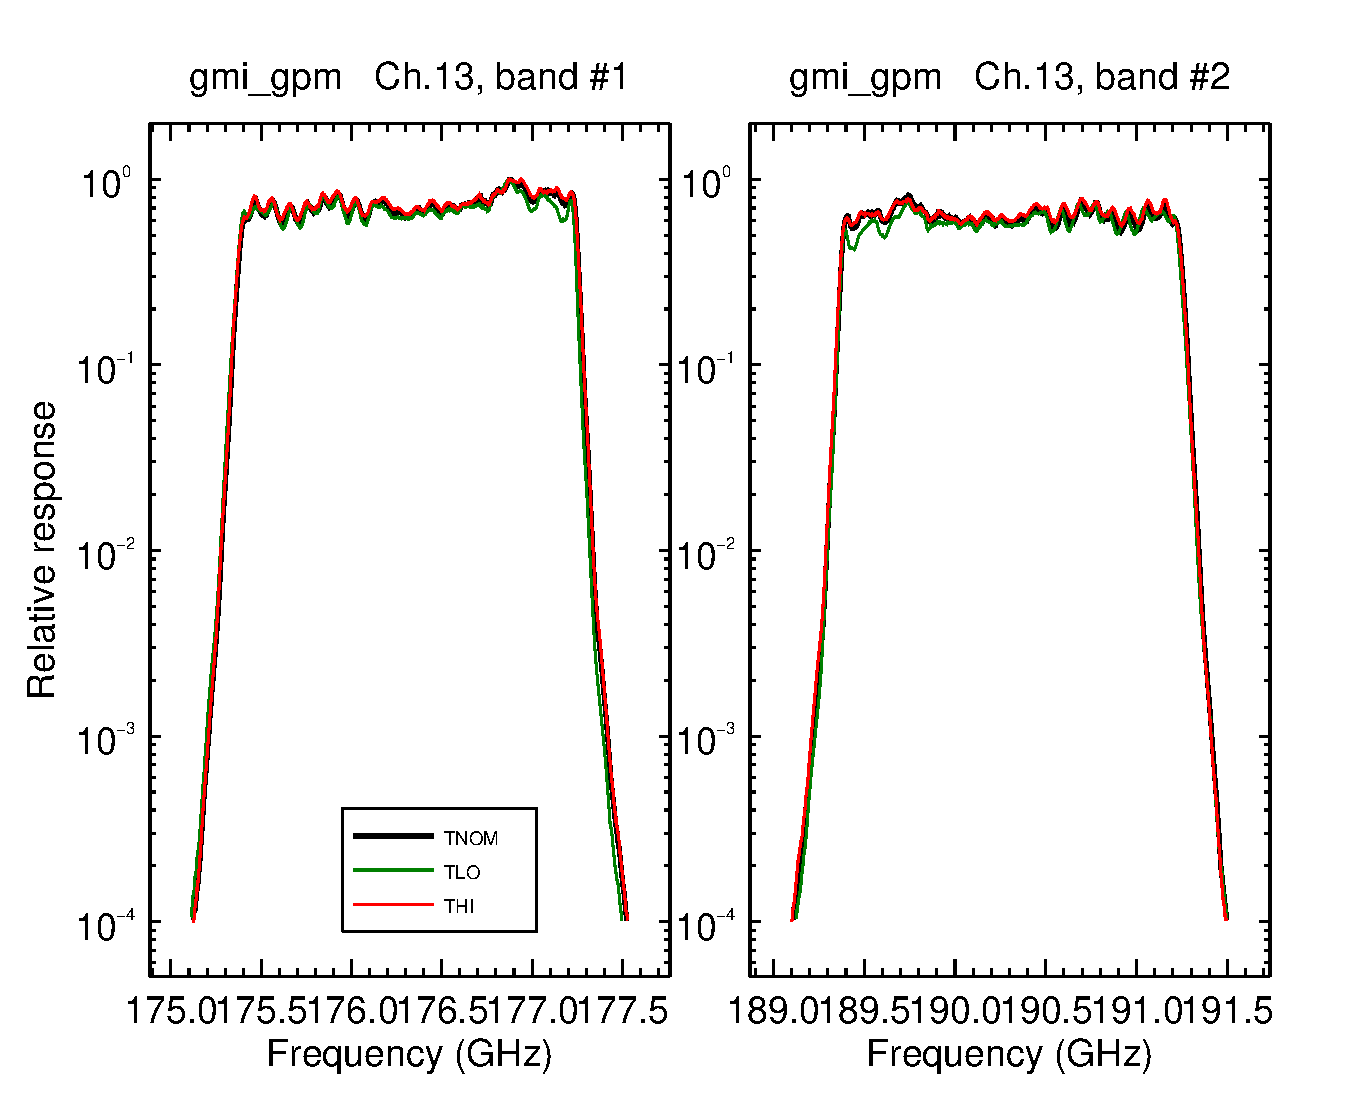
\includegraphics[scale=0.3]{graphics/log/gmi_gpm-13.eps}
  \end{tabular}
  \caption{GMI channel 13 responses for the three test temperatures: $T_{NOM}$ (25\textdegree{}C), $T_{LO}$ (-10\textdegree{}C), and $T_{HI}$ (45\textdegree{}C). \textbf{(Left)} Linear y-axis. \textbf{(Right)} Base-10 logarithmic y-axis.}
  \label{fig:ch13_response}
\end{figure}

